\documentclass{article}
\usepackage{graphicx}
\usepackage{sidecap}
\usepackage{float}
\usepackage{subcaption}
\usepackage{blindtext}
\usepackage{apacite}
\usepackage{colortbl}
% if you need to pass options to natbib, use, e.g.:
%     \PassOptionsToPackage{numbers, compress}{natbib}
% before loading neurips_2018

% ready for submission
% \usepackage{neurips_2018}

% to compile a preprint version, e.g., for submission to arXiv, add add the
% [preprint] option:
%     \usepackage[preprint]{neurips_2018}

% to compile a camera-ready version, add the [final] option, e.g.:
     \usepackage[final]{final_project}

% to avoid loading the natbib package, add option nonatbib:
%     \usepackage[nonatbib]{neurips_2018}

\usepackage[utf8]{inputenc} % allow utf-8 input
\usepackage[T1]{fontenc}    % use 8-bit T1 fonts
\usepackage{hyperref}       % hyperlinks
\usepackage{url}            % simple URL typesetting
\usepackage{booktabs}       % professional-quality tables
\usepackage{amsfonts}       % blackboard math symbols
\usepackage{nicefrac}       % compact symbols for 1/2, etc.
\usepackage{microtype}      % microtypography

\title{Identifying Hand Gestures through Myographic Signals via ANN}

% The \author macro works with any number of authors. There are two commands
% used to separate the names and addresses of multiple authors: \And and \AND.
%
% Using \And between authors leaves it to LaTeX to determine where to break the
% lines. Using \AND forces a line break at that point. So, if LaTeX puts 3 of 4
% authors names on the first line, and the last on the second line, try using
% \AND instead of \And before the third author name.

\author{%
  Eduardo Coronado\ \\
  Duke University \\
  % examples of more authors
  \And
   Sebastian Knigge \\
   Duke University \\
  % Address \\
  % \texttt{email} \\
  \AND
  Sam Voisin \\
  Duke University \\
  % Address \\
  % \texttt{email} \\
  \And
  Yuan Zheng \\
  Duke University \\
  % Address \\
  % \texttt{email} \\
  % \And
  % Coauthor \\
  % Affiliation \\
  % Address \\
  % \texttt{email} \\
}

% Comments
\newtheorem{com}{Comment}

\begin{document}
% \nipsfinalcopy is no longer used

\maketitle

\begin{abstract}
 In this paper we develop a series of artificial neural networks (ANNs) for predicting hand gestures through nerve impulses detected by sensors placed on the forearms of a series of test subjects. We then compare these ANNs based on their accuracy, the time it takes to fit the models, and their overall complexity with the ultimate goal of determining the best model for use in the next generation of automated prosthetics. Dimension reduction techniques are also used in the modeling process with models fitted using a subset of the principal components compared to their higher dimension counterparts.
\end{abstract}

\section{Introduction}
In recent decades, advances in surface electromyographic signals (sEMG) recording systems have allowed researchers to determine the distinct groups of muscles involved in certain movements. \footnote{\cite{bishop2004}}, \footnote{\cite{winter1991}}  Patterns found in these recordings have further enabled the classification  of certain movements distinct movements, which have led to the development and use sEMG-based human-machine interfaces. Recent advances in sEMG analytics methods have encouraged the use of these type of muscular signals in human-machine interfaces used to control exoskeletons and protheses; however, challenges remain.\footnote{\cite{Sensorpaper}} \footnote{\cite{kiguchi2012}} \footnote{\cite{roche2014}}

These challenges are related the accuracy of motion recognition that different pattern classification methods can achieve, which tends to be highly variable. Although classification has mostly done via linear discriminant analysis (LDA), other methods that are commonly used in the field are support vector machines (SVMs) and Artificial Neural Networks (ANN). \footnote{\cite{LDA}} \footnote{\cite{ANN}}   Overall, these methods have shown to have a high accuracy of simple body movements. However, given user movements are highly variable the accuracy greatly varies and can be suboptimal. Additionally, there is inherent noise of sEMG recording systems and user-specific anatomical characteristics that need to be considered. \footnote{\cite{emgnoise}}    In turn, these factors lead to downstream problems when attempting to convert these classifications into spatial directions (e.g. up, down, right, and left). Therefore, these challenges have greatly limited the deployment of human-machine interface systems for wider commercial use.

In this paper, we aim to address the former challenge of accuracy via ANN. Our goal is to design and implement a light-weight supervised learning model via a multi-layered neural network to accurately identify six distinct hand gestures from Lobov \textit{et al}  sEMG data. footnote{\cite{Sensorpaper}} Our approach focuses on first determining the most relevant principal components from this  multi-channeled dataset, and then assess the performance of multi-layered neural networks based on their accuracy vs computational time..

\section{Methods}
\label{Methods}


\subsection{Workflow Overview}
For this project our workflow was comprised of 4 main phases: preprocessing, dimension reduction via PCA, modeling, and performance comparison as shown in Figure \ref{Flow} below. 

\begin{SCfigure}[][h]
  \centering
  \caption{Schematic of overall workflow stages: preprocessing, PCA, modeling and performance comparison}
  \includegraphics[width=0.5\textwidth]%
    {Graphics/Flow}% picture filename
    \label{Flow}
\end{SCfigure}


\subsection{sEMG Data}
Raw sEMG signal data from 36 individuals was obtained online from Lobov et al \footnote{Ibid}. Two series were recorded per individual, each comprised of signals obtained via 8 equally spaced sensors around the forearm (i.e. channels). For each series, subjects were asked to performed a set of 6 basic hand gestures. Each gesture was performed for 3 seconds with a 3 second pause in between. Gestures classification scheme is shown in Table 1. 

\begin{figure}[!htb]
  \centering
  \captionsetup{labelformat=empty}
\caption{Table 1. sEMG gesture classifications}
  \includegraphics[width=0.8\textwidth]%
    {Graphics/table1}% picture filename
\end{figure}



\subsection{Preprocessing}

We implemented a root means squared (RMS) envelope of $200$ ms overlapping time windows at $100$\textit{ms} steps via the \textit{biosignalEMG} R package\footnote{\cite{biosignalEMG}} to remove some of the noise generated during sEMG signal collection. As shown in Figure \ref{fig:Smooth} the pre-processing does help provide a means to generate clearer signals that show distinct patterns from each channel per gesture

\begin{figure}[H]
  \centering
  \caption{Schematic of overall workflow stages: preprocessing, PCA, modeling and performance comparison}
  \includegraphics[width=0.9\textwidth]%
    {Graphics/smooth_ex}% picture filename
    \label{fig:Smooth}
\end{figure}

Subsequently, the data was separated according to the gesture classifications (1-6) provided for each time step for further analysis.

\subsection{Dimension Reduction}

Dimension reduction for each gesture was done via a principal component analysis (PCA) of the 8 distinct channels used to record sEMG data in order to identify the most relevant channels for gesture classification and potentially  reduce the training time of the neuronal network. We achieved this via the R \textit{princomp} function that performs a spectral decomposition via singular value decomposition (1) of the gesture design matrix ($\mathbf{X}$)
\begin{equation}
\mathbf{X = U D V'}
\end{equation}
were $U$ and $V$ are the row and column space eigen vectors and $D$ is a diagonal matrix with the eigen values.

\subsection{Modeling}

Before fitting an Artificial Neural Network (ANN) we "padded" the ends of each gesture's data matrix to ensure that the vectors passed into the models are of equal dimension. We then developed two ANN with one hidden layer, the first with all components and a second with channels subset selected during the dimension reduction stage (Figures  \ref{fig:1Layer} and \ref{fig:PCA1Layer}, respectively ). Each of these has a single hidden layer with eight hidden nodes having linear activation. These eight nodes feed into six output nodes with a soft-max activation function. This model was inspired by Lobov et al's approach.\footnote{\cite{Sensorpaper}}

\begin{figure}[h]
\centering
\begin{subfigure}{.5\textwidth}
  \centering
  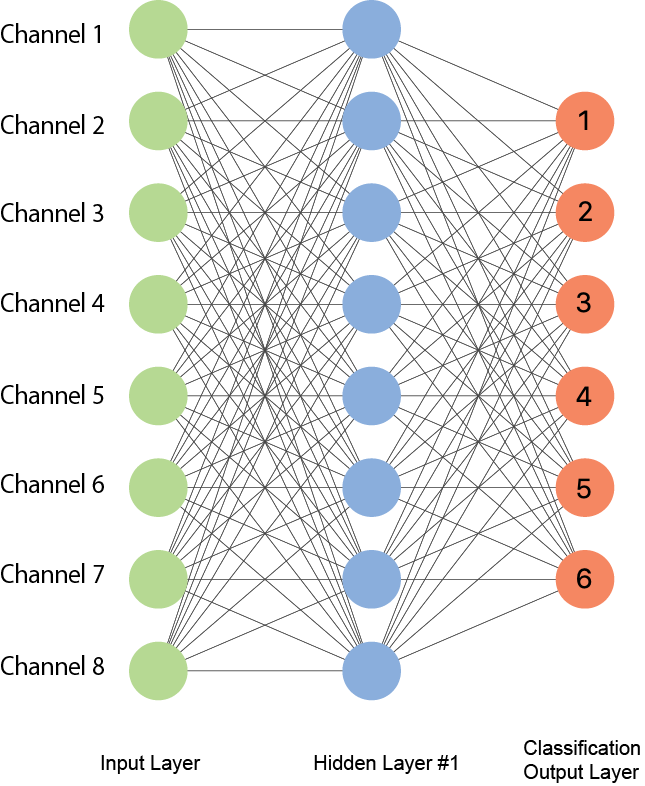
\includegraphics[width=.9\linewidth]{Graphics/1-layer-NN}
  \caption{Schematic of ANN with all 8 channels }
  \label{fig:1Layer}
\end{subfigure}%
\begin{subfigure}{.6\textwidth}
  \centering
  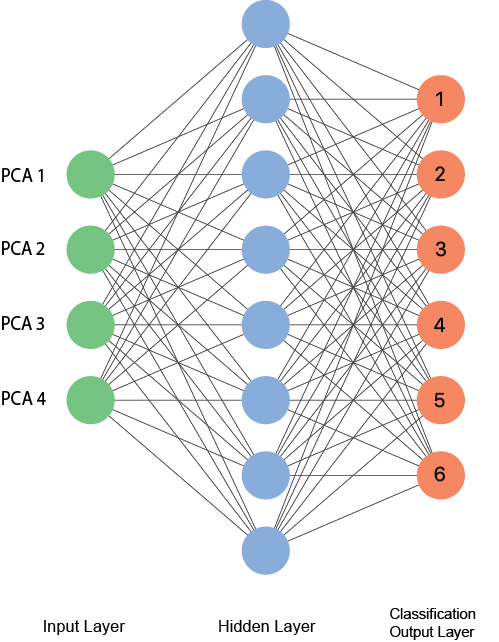
\includegraphics[width=.7\linewidth]{Graphics/1-layer-PCA-NN}
  \caption{Schematic of ANN with 4 PC channels}
  \label{fig:PCA1Layer}
\end{subfigure}
\caption{Artificial Neuronal Net structures}
\label{gig:Model}
\end{figure}

The  computation graphs for the ANN were generated via an R implementation of Keras\footnote{\cite{Keras}}, which relies on Google's TensorFlow engine for backpropogation. This allowed us to implement a flexible design framework so that we could  add, edit, and remove layers from our models quickly and efficiently during our development process. \\
Afterward, five additional ANN were generated with an increasing number of hidden layers ($l=1,...5$) but only using the principal components as inputs. Figure \ref{fig:5Layers} shows a schematic representation of how each hidden layer was added following a similar process for inputs and outputs as for the initial ANNs.

\begin{figure}[h]
\centering
\begin{subfigure}{.5\textwidth}
  \centering
  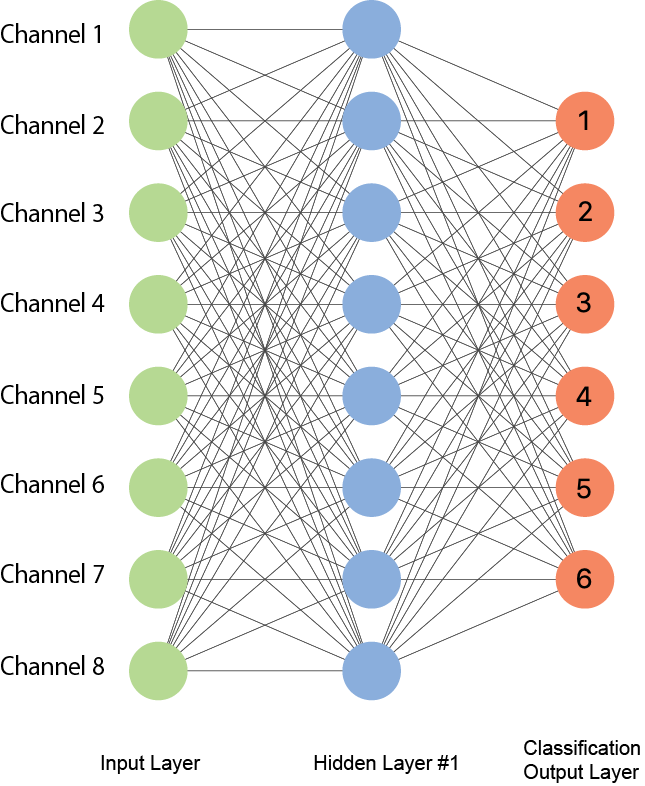
\includegraphics[width=.8\linewidth]{Graphics/1-layer-NN}
\end{subfigure}%
\begin{subfigure}{.6\textwidth}
  \centering
  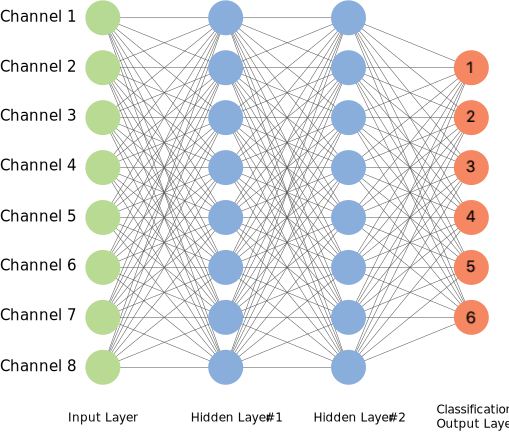
\includegraphics[width=.9\linewidth]{Graphics/2-layer-NN}
\end{subfigure}
\caption{Increasing number of hidden layers in Artificial Neuronal Net structure}
\label{fig:5Layers}
\end{figure}

\subsection{Performance Assessment}
To assess the performance of each ANN, we used an k-fold cross validation strategy ($k =5$) to split our data to generate a gesture-specific training and a testing sets. These were using the \textit{caret} R package via random sampling. We then assessed the average classification accuracy of each ANN using a categorical cross entropy metric which measures the \textit{Kullback-Leibler} (KL) divergence between the true distribution of the response variable and the distribution of the predictions. This was done for both the initial ANN previously mentioned and shown in Figures \ref{fig:1Layer} and \ref{fig:PCA1Layer}, as well the subsequent ANN with increasing number of layers from Figure \ref{fig:5Layers}.\\
Additionally, our code was timed to assess the computational costs versus gains in accuracy as we increase the number of layers.


\section{Results}

\subsection{Principal Component Analysis}

Using the spectral decomposition we found that only $4$ of the $8$ principal components in our dataset contributed meaningfully to variance in our response. From figure $3$, we can see that these $4$ components account for approximately $80$\% of the variability we are seeking to model.\\
We might be interested in comparable results, or a decision rule which is applicable to different data sets. We introduce a relative measure $\kappa$ which can be used for the PCA of data sets with any dimension. Let $p$ be the number of dimensions of the original data set.

\[\kappa_i=\frac{{proportional\ explained\ variance}_i}{\frac{1}{p}}={proportional\ explained\ variance}_i\times p\]

for $i=1,...,p$.

One can define a decision rule, which is dependent on a threshold $\delta$: \textit{Include $PC_i \ \forall \ \kappa_i>\delta$}

For our data set we choose $\delta:=0.6$.

\begin{figure}[H]
  \centering
  \caption{PCA Screeplot and cumulutive variance plot}
  \includegraphics[width=0.9\textwidth]%
    {Graphics/PCA_Plots/PCA_screeplot-150dpi}% picture filename
    \label{fig:PCA}
\end{figure}

% Table created by stargazer v.5.2.2 by Marek Hlavac, Harvard University. E-mail: hlavac at fas.harvard.edu
% Date and time: Do, Apr 25, 2019 - 14:58:37
\begin{table}[!htbp] \centering 
  \caption{PCA measures} 
  \label{} 
\begin{tabular}{@{\extracolsep{0pt}} ccccccccc} 
\\[-1.8ex]\hline 
\hline \\[-1.8ex] 
 & Comp. 1 & Comp. 2 & Comp. 3 & Comp. 4 & Comp. 5 & Comp. 6 & Comp. 7 & Comp. 8 \\ 
\hline \\[-1.8ex] 
proportion of \\  explained variance & $0.343$ & $0.211$ & $0.132$ & $0.116$ & $0.072$ & $0.055$ & $0.043$ & $0.028$ \\ 
\hline \\
cummulative explained \\ variance & $0.343$ & $0.554$ & $0.686$ & $0.802$ & $0.874$ & $0.929$ & $0.972$ & $1$ \\ 
\hline \\
$\kappa$ & $2.744$ & $1.689$ & $1.056$ & $0.930$ & $0.574$ & $0.437$ & $0.345$ & $0.225$ \\ 
\\[-1.8ex]\hline 
\hline \\[-1.8ex] 
\end{tabular} 
\end{table} 


By reducing the number of inputs from $8$ smoothed signals to only $4$ principle components, we were able to reduce overfitting in our model prior to utilizing any dropout layers. This reduction in overfitting decreased prediction accuracy in the validation data set only slightly see the \textit{ANN Performance Comparison} section.


\subsection{ANN Performance Comparison}
First we compare the time and validation accuracy for 1 layer Neural Netwrok using 4 components and 8 components to get the taste of the advantage of using PCA.

\begin{table}[!htbp] \centering 
  \caption{4 Principal Components and 8 Principal Components Comparison} 
  \label{tab:PCA48} 
\begin{tabular}{@{\extracolsep{0pt}} ccccccccc} 
\\[-1.8ex]\hline 
\hline \\[-1.8ex] 
 & 4 Principal Components Analysis & 8 Principal Components Analysis \\ 
\hline \\[-1.8ex] 
Training Time \\  System Time & $62.622s$ & $78.302s$\\ 
\hline \\
Accuracy \\ On Validation Dataset & $0.775$ & $0.809$ \\ 
Ratio of change in accuracy\\ to change in time & $ \texttt{\char`\~}$ & $0.002$ \\ 
\\[-1.8ex]\hline 
\hline \\[-1.8ex] 
\end{tabular} 
\end{table} 

\begin{figure}[H]
  \centering
  \caption{1 Layer NN with 4 Principal Components}
  \includegraphics[width=0.5\textwidth]%
    {Graphics/4PC_Avg_CV_ANN_1_layers}% picture filename
    \label{fig:4PC}
\end{figure}

\begin{figure}[H]
  \centering
  \caption{1 Layer NN with 8 Principal Components}
  \includegraphics[width=0.5\textwidth]%
    {Graphics/4PC_Avg_CV_ANN_1_layers}% picture filename
    \label{fig:8PC}
\end{figure}

From the timing and accuracy table for 4PC and 8PC (Table \ref{tab:PCA48}) as well as two plots above (Figure \ref{fig:4PC} and \ref{fig:8PC}), we can see that in one layer Neural Network, the training time using 4PC is much less than that using 8PC (or the whole information), which means that this data reduction helps decrease much computation intensity when training models. Besides, by comparing their classification accuracy on the validation dataset, using 4PC only sacrifice little on the performance of the model, the ratio of change in accuracy to change in time is only 0.002.\newline

After balancing the gain and loss, we decide that training model with 4 PC is a better choice, because it's much less computational intense while maintain the most part of the information in the original data as well as high performance on the model. In fact, it is not necessary to presume such little more accuracy at the price of so much time and computation intensity.\newline

Next we train our model using 4PC with different number of layers and results are as following:



\begin{table}[!htbp] \centering 
  \caption{Timing and Accurary} 
  \label{} 
\begin{tabular}{@{\extracolsep{0pt}} ccccccccc} 
\\[-1.8ex]\hline 
\hline \\[-1.8ex] 
 & One Layer & Two Layers & Three Layers & Four Layers & Five Layers  \\ 
\hline \\[-1.8ex] 
Training Time \\  System Time & $55.267s$ & $77.497s$ & $90.501s$ & $110.841s$ & $122.357s$ \\ 
\hline \\
Accuracy \\ On Validation Dataset & $0.750$ & $0.735$ & $0.715$ & $0.720$ & $0.655$  \\ 
Ratio of change in accuracy\\ to change in time & $ \texttt{\char`\~}$ & $-0.0006$ & $-0.015$ & $0.002$ & $-0.005$  \\ 
\\[-1.8ex]\hline 
\hline \\[-1.8ex] 
\end{tabular} 
\end{table} 

\begin{figure}[H]
  \centering
  \caption{One Layer Accuracy}
  \includegraphics[width=0.5\textwidth]%
    {Graphics/Avg_CV_ANN_1_layers}% picture filename
    \label{fig:1 layer}
\end{figure}

\begin{figure}[H]
  \centering
  \caption{Five Layers Accuracy}
  \includegraphics[width=0.5\textwidth]%
    {Graphics/Avg_CV_ANN_5_layers}% picture filename
    \label{fig:5 layer}
\end{figure}

From the timing and accuracy table for every number of layers (layer) and two plots above, we can see that the most time-wasting method is 5 layers ANN, which will take about 122s on the training, while the fastest method is 1 layer ANN, which only takes about 55s on the same training dataset. This result is not surprising because as we add more layers, the computation intensity increases at the same time. \newline
Now considering the classification accuracy, it turns out that one layer Neural Network has the highest accuracy on validation dataset and the performance doesn't improve when adding more layers but become worse sometimes.\newline
Another thing that is worth to point out is that when doing validation, the accuracy on the validation dataset exceeds that on the training set and this kind of thing doesn't always happen. It is partly because of the characteristic of our dataset. Since it highly depends on time sequence, the training dataset and validation dataset are highly correlated and we may have underfitting on the training set.


\section{Conclusion}
Through the analysis and modeling procedures described above, we have shown that it is possible to predict gestures using using artificial neural networks trained on sEMG signals data. Although increasing the number of dense hidden layers in the network did not result in greater predictive power, we were able to reduce the computational cost of fitting the ANN using a conceptually simple spectral decomposition for dimension reduction.

This result is important because it not only serves to validate some of the results of the original research performed by Lobov \textit{et al} but it also demonstrates that they could have achieved similar accuracy with a less complex model through some standard dimension reduction techniques. Furthermore, our work shows that the next generation of prosthetics and exoskeletons can be equipped with sensors to record sEMG signals and pre-trained ANNs that are capable of responding to the user's nervous impulses in an intelligent, automated manner. However, the user-specific anatomy will remain as a current limitation to the accuracy of ANN implemented. Furthermore, we believe that the results presented here can be improved upon through further experimentation into recurrent neural network models and  more specialized hardware to this task.




\newpage





\bibliographystyle{apacite}

\bibliography{References}



\end{document}